\documentclass[12pt, titlepage]{article}
\usepackage[shortlabels]{enumitem}
\usepackage{booktabs}
\usepackage{graphicx}
\usepackage{tabularx}
\usepackage{lscape}
\usepackage{hyperref}
\usepackage{float}
\usepackage{longtable}
\usepackage{geometry}
\hypersetup{
	colorlinks,
	citecolor=black,
	filecolor=black,
	linkcolor=red,
	urlcolor=blue
}
\usepackage[round]{natbib}
\title{SE 4G06: Software Requirements Specification\\\progname}

%\author{Team \#, Team Name
%	\\ Faiq Ahmed
%	\\ Student 2 name and macid
%	\\ Student 3 name and macid
%}

\author{\authname}

%% Comments

\usepackage{color}

\newif\ifcomments\commentstrue %displays comments
%\newif\ifcomments\commentsfalse %so that comments do not display

\ifcomments
\newcommand{\authornote}[3]{\textcolor{#1}{[#3 ---#2]}}
\newcommand{\todo}[1]{\textcolor{red}{[TODO: #1]}}
\else
\newcommand{\authornote}[3]{}
\newcommand{\todo}[1]{}
\fi

\newcommand{\wss}[1]{\authornote{blue}{SS}{#1}} 
\newcommand{\plt}[1]{\authornote{magenta}{TPLT}{#1}} %For explanation of the template
\newcommand{\an}[1]{\authornote{cyan}{Author}{#1}}

%% Common Parts

\newcommand{\progname}{ProgName} % PUT YOUR PROGRAM NAME HERE
\newcommand{\authname}{Team \#, Team Name
\\ Student 1 name and macid
\\ Student 2 name and macid
\\ Student 3 name and macid
\\ Student 4 name and macid} % AUTHOR NAMES                  

\usepackage{hyperref}
    \hypersetup{colorlinks=true, linkcolor=blue, citecolor=blue, filecolor=blue,
                urlcolor=blue, unicode=false}
    \urlstyle{same}
                                


\date{\today}
\begin{document}
	
	\maketitle
	
	\pagenumbering{roman}
	\tableofcontents
	\listoftables
	\listoffigures
	
	\begin{table}[H]
		\caption{\bf Revision History}
		\begin{tabularx}{\textwidth}{p{3cm}p{2cm}X}
			\toprule {\bf Date} & {\bf Version} & {\bf Notes}\\
			\midrule
			October 4th & 1.0 & Introduction added by Eesha\\
			October 4th & 1.1 & Functional requirements started by Faiq and Veerash\\
			October 4th & 1.2 & Nonfunctional requirements started by Kevin\\
			October 5th & 1.3 & Project Issues added by Faiq and Veerash \\
			October 5th & 1.4 & Functional requirements finished and revised \\
			October 5th & 1.5 & Non functional requirements finished and revised \\
			October 5th & 1.6 & Appendix added\\
			October 5th & 1.7 & Traceability matrix added\\
			\bottomrule
		\end{tabularx}
	\end{table}
	
	\newpage
	
	\pagenumbering{arabic}
	
	\section{Changes to template}
	
	The template was changed to include separate sections for main requirements and requirements for undesired events in the functional requirements section to create a better distinction between them and make the template easier to follow. Additionally sections to make a distinction between likely and unlikely changes in the functional requirements and rationale for specific requirements were also added. Lastly, additional sections to include the traceability matrix and phase in plan were added as they were missing from this template.
	
	\section{Project Drivers}
	
	\subsection{The Purpose of the Project}
	
	The purpose of this project is to create a collaborative \textbf{LaTex} editing and compiling software that supports version control with\textbf{ Git }integration. The software will allow for multiple members of a team to view, edit and compile the same\textbf{tex}files at the same time while seeing the changes made by others in real time. This is especially useful for teams preparing project documentation where multiple members need to contribute to the documents in parallel, however it is widely intended for the development of any \textbf{LaTex} document by any number of contributors for any reason.\\
	\\The \textbf{LaTex} editor will support version control management through\textbf{ Git }integration so that the version history of any document created will be easily accessible. This is especially useful for documents that are likely to change over time due to revisions, such as software documentation and release notes
	
	
	\subsection{The Stakeholders}
	
	\subsubsection{The Client}
	
	The client of this software is Dr.Spencer Smith who has requested the development of this project for the software engineering Capstone course in order to solve a real world problem. The clients also include enterprises and companies that are seeking a standardized documentation software to prepare internal documents across teams who possess \textbf{LaTex} proficiency.
	
	\subsubsection{The Customers}
	The customers are the purchasers and users of this software. This includes individuals who wish to install the software for their personal use, students who wish to use the software for individual or team projects, companies and teams who wish to purchase a license and anyone else interesting in using the\textbf{tex}editor.\\
	Customers also include researchers, developers, and other secondary customers of the software such as employees of a company that chooses to make use of the software for their teams. Such employees will be interested in the usability and features of the product. Researchers and developers who are interested in the expansion of the document editor market or the development of such softwares are included in the stakeholders.\\
	
	\subsubsection{Other Stakeholders}
	Other stakeholders also include the primary developers and testers of this software, namely Faiq Ahmed, Eesha Qureshi, Veerash Palanichamy, and Kevin Kannammallil as their software engineering skills are a resource invested in this software and they are concerned in the outcome of this project.
	
	\subsection{Mandated Constraints}
	
	\begin{enumerate}[{MC}1.]
		\item Project must be completed by April 2023
		\\Rationale: Project must adhere to Capstone 4G06 timeline
	\end{enumerate}
	
	\subsection{Naming Conventions and Terminology}
	
	\begin{itemize}
		\item \textbf{LaTex}:A document preparation system and language
		\item \textbf{Tex}: A shorthand for \textbf{LaTex}
		\item \textbf{Git}: A version control software
		\item \textbf{GitHub} A propriety hosting software for \textbf{git} version control
		\item \textbf{Commit}: A snapshot or the creation of a snapshot of a project that is stored in a commit history log and can be viewed at any time
		\item \textbf{Repository}: Central location where all \textbf{git} version history of data is stored
		\item \textbf{PDF}: A printable document file
		\item \textbf{API}: An interface between two services
		\item \textbf{JSON Web Tokens}: Compact tokenized methods of verifiable data transfer that use JavaScript string object notation
	\end{itemize}
	
	\subsection{Relevant Facts and Assumptions}
	
	\begin{enumerate}
		\item Users are proficient with \textbf{LaTex}
		\item Users are proficient with \textbf{Git}
		\item The system will validate that a user is logged in
		\item The system will create a \textbf{Git} repository for new projects
		\item Users will be operating on a Chrome, Firefox or Safari web browser
	\end{enumerate}
	
	\section{Functional Requirements}
	
	\subsection{The Scope of the Work and the Product}
	
	\subsubsection{The Context of the Work}
	
	\subsubsection{Context Diagram}
	
	\begin{figure}[H]
		\centering
		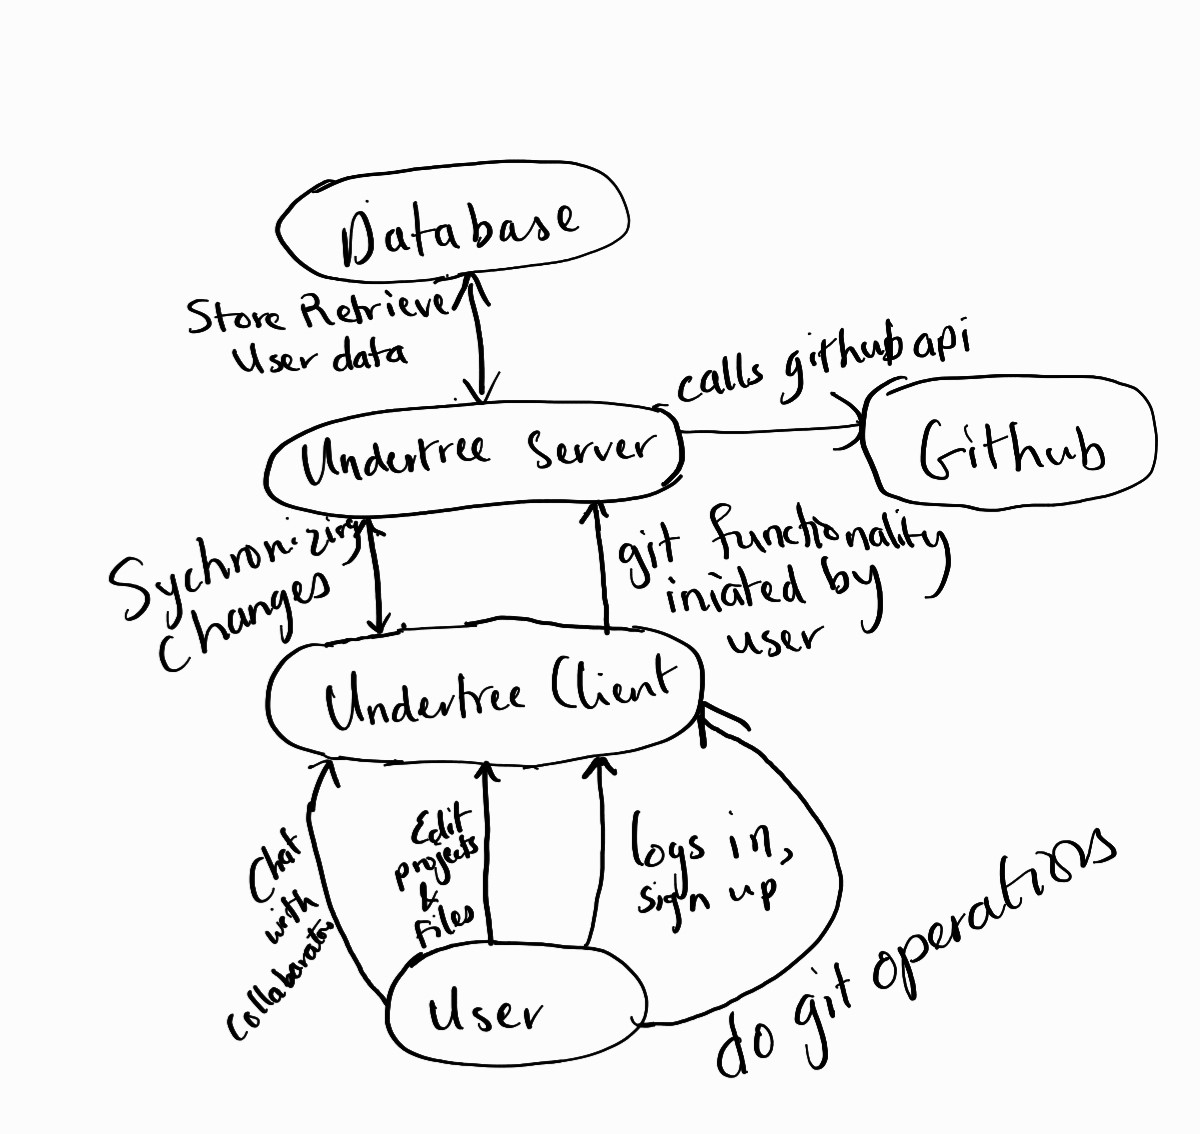
\includegraphics[scale=0.4]{context.jpg}
		\caption{Context Diagram of UnderTree}
	\end{figure}
	\newpage
	\subsubsection{Work Partitioning}
	
	\begin{longtable}{|p{4cm}|p{5cm}|p{5cm}|}
		\hline
		\textbf{Event Name} & \textbf{Input/Output} & \textbf{Summary} \\
		\hline
		1. Log in & \textbf{Input:} \textbf{GitHub} Username, \textbf{GitHub} Password \newline \textbf{Output:} New access permissions related to the account & The user will need to log in with their \textbf{GitHub} account to get access to their private projects and be able to edit them with collaborators.\\
		\hline
		2. Create project & \textbf{Input:} Project name and collaborators \newline \textbf{Output:} Access to the new project and a new \textbf{Git} repository for the project & Users will need to create a project to work on the \textbf{LaTex} files.\\
		\hline
		3. Import Project & \textbf{Input:} Select \textbf{Git} repository \newline \textbf{Output:} A new project with the data from the repository & The user may want to import existing repositories\\
		\hline
		4. Delete Project & \textbf{Input:} Mouse click to delete project and mouse click to confirm delete \newline \textbf{Output:} Remove the project from the user and all collaborators accounts & The user may want to remove a project from their accounts\\
		\hline
		5. Edit Project & \textbf{Input:} Collaborator's Id to add to project \newline \textbf{Output:} New collaborator in project & Users may want to add more collaborators to the project.\\
		\hline
		6. View all projects & \textbf{Input:} Open project menu \newline \textbf{Output:} Display a list of all projects and their names & User will want to see a list of all their existing projects\\
		\hline
		7. Create a file & \textbf{Input:} File name \newline \textbf{Output:} New file in project & This allows user to add files to a project\\
		\hline
		8. Delete a file & \textbf{Input:} Click delete button  \newline \textbf{Output:} Remove file from project &  Users may wish to remove existing files from a project.\\
		\hline
		9. Edit file  & \textbf{Input:} Text to add, remove or modify \newline \textbf{Output:} Updated changes in the file &  Adding new changes to the file should be reflected to all users\\
		\hline
		10. View file & \textbf{Input:} Click button to open file \newline \textbf{Output:} Display all users cursors and live changes happening to the file &  Users should be able to see the changes happening to the file in real time\\
		\hline
		11. View revision history & \textbf{Input:} Click button to see revision history \newline \textbf{Output:} Display all revisions as well as users responsible for each revision &  Users should be able to see \textbf{commit} history and how file was changed over time\\
		\hline
		12. \textbf{Commit} changes & \textbf{Input:} Select sections to \textbf{commit} and add a message for the \textbf{commit} \newline \textbf{Output:} All changes to the project reflected in \textbf{Git} repository &  Users should be able to reflect the changes from the project into the corresponding \textbf{Git} repository\\
		\hline
		13. Send chat message & \textbf{Input:} Type chat message and click the send button \newline \textbf{Output:} Chat message should be sent and visible to other users &  Users should be able to communicate with each other over the chat\\
		\hline
		14. View chat messages & \textbf{Input:} Open the chat \newline \textbf{Output:} All chat messages sent by other &  Users should be able to see all messages sent by other users in the project\\
		\hline
		\caption{Work Partitioning Events and Summaries}
	\end{longtable}
	\newgeometry{left=5mm, top=25mm} 
	\subsubsection{Individual Product Use Cases}
	\begin{figure}[H]
		\centering
		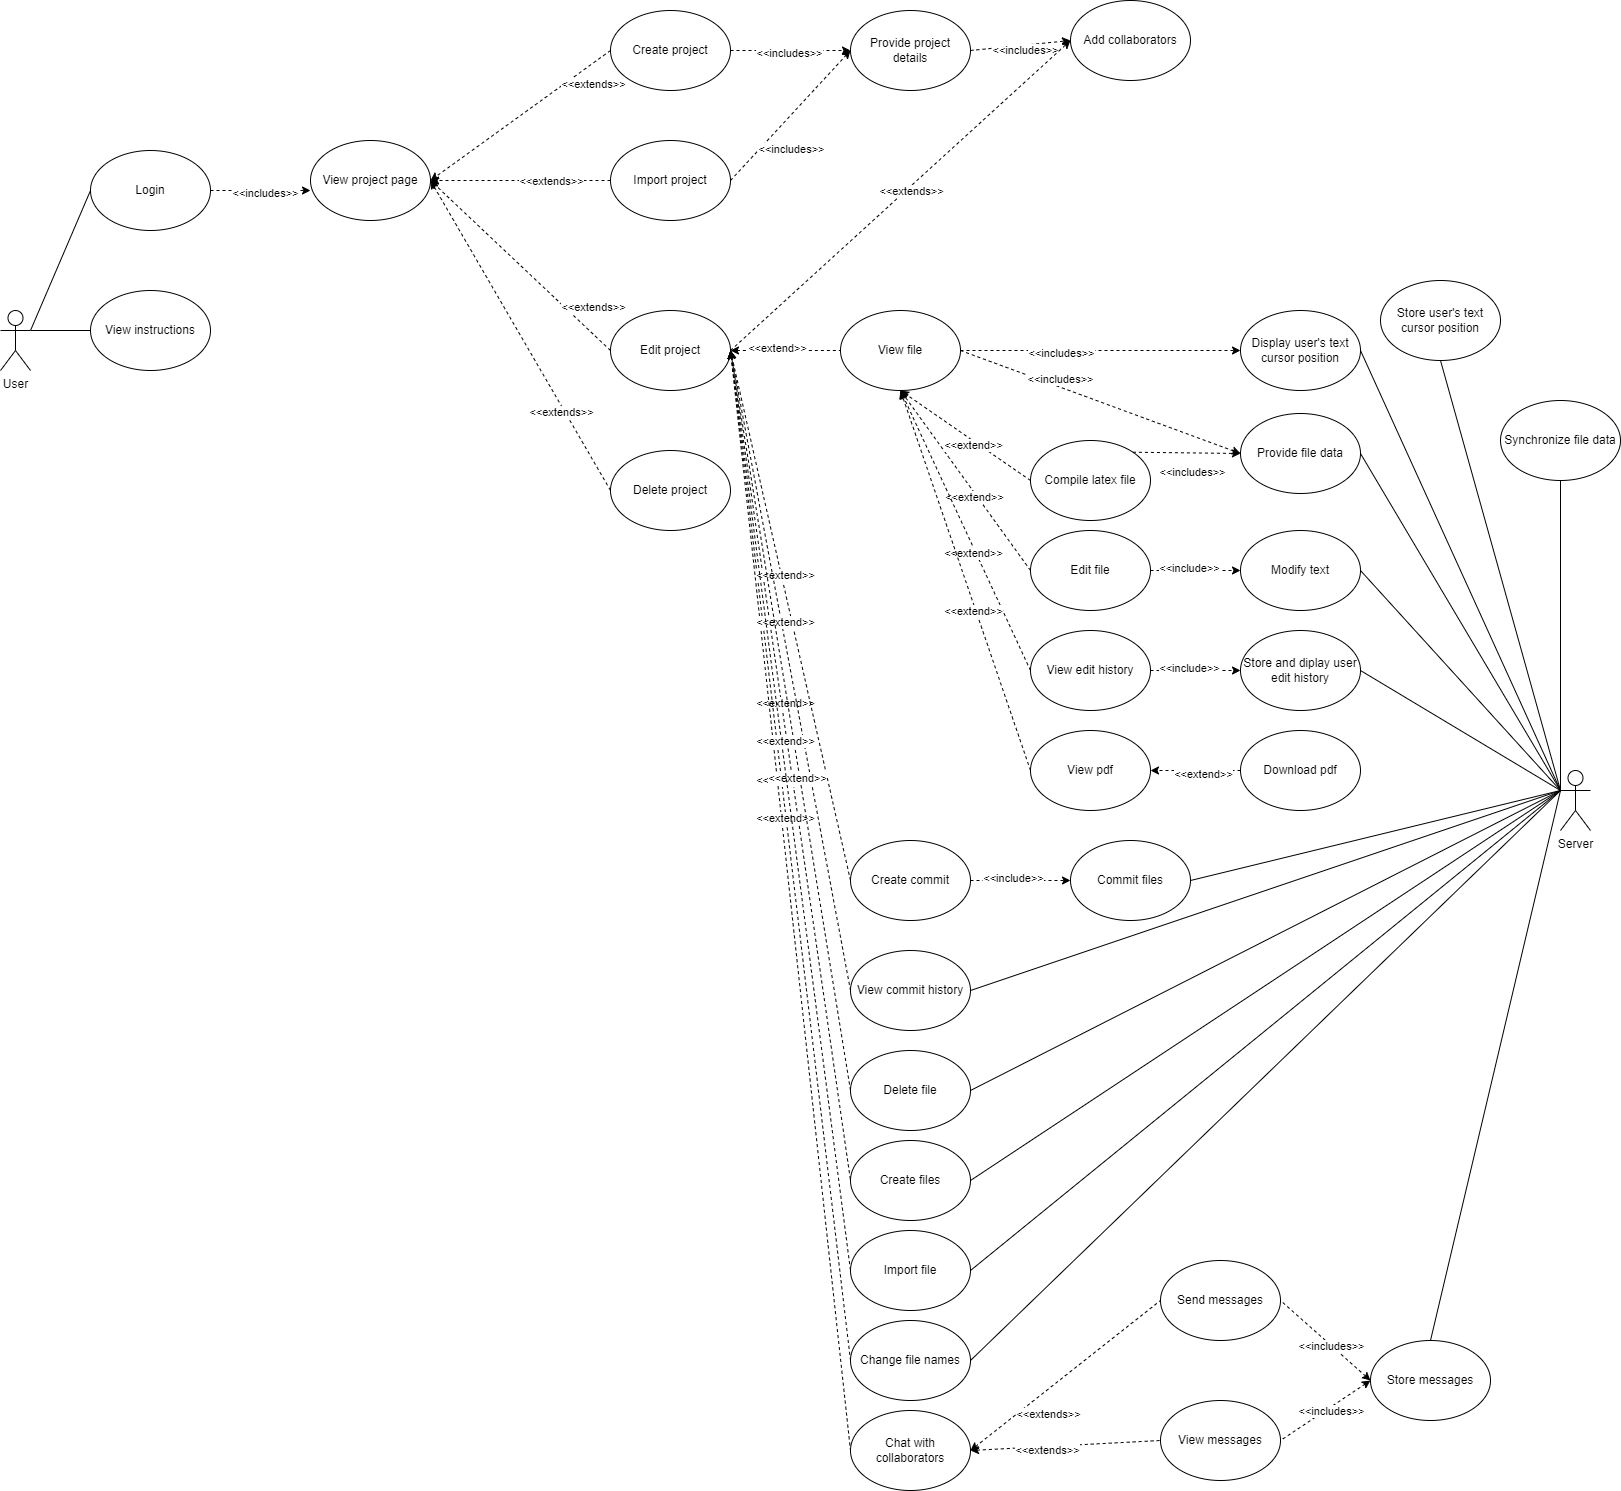
\includegraphics[scale=0.35]{use_case.png}
		\caption{Use case diagram for UnderTree, \href{https://drive.google.com/file/d/1Qnl_AmKnUPbMSakRkb6BuVxByL-jOyM9/view?usp=sharing}{Link to draw.io}}
	\end{figure}
	\restoregeometry
	
	\subsection{Functional Requirements}
	
	\subsubsection{Main Requirements}
	
	\textbf{To avoid repetition in the functional requirements for all functional requirements after log in, assume that the system checks to ensure that the user is logged in and has appropriate access level.}\\
	
	\noindent \textbf{Formal Specification Variables:}
	
	\noindent \textbf{change}: This is a specific datatype that stores changes made by a spefic user.
	
	\noindent \textbf{all\_changes}: This is an array of changes that stores all changes made in a file in order.
	
	\noindent \textbf{user\_changes}: This is an array of changes specific to a user in a specific file.\\
	
	\begin{enumerate}[{BE}1.]
		\item The user wants to view instructions
		\begin{enumerate}[{FR}1.]
			\item The system must allow the user to be able to open and view instructions
			\item The system must allow the user to close the instructions and return to their previous task
		\end{enumerate}
		\item The user wants to login to their account
		\begin{enumerate}[resume*]
			\item The system must allow the user to log into the system with a unique \textbf{Git} identity
			\item The system must validate the identity of the user
		\end{enumerate}
		\item The user wants to create a project 
		\begin{enumerate}[resume*]
			\item The system must allow the user to pick the project name
			\item The system must allow the user to add collaborators to the project
			\item The system must create a \textbf{Git} repository for the project
		\end{enumerate}
		\item The user wants to import a project
		\begin{enumerate}[resume*]
			\item The system must ask user to choose a repository to import
			\item The system must import all\textbf{tex}file in the repository
			\item The system must import all collaborators from the repository
		\end{enumerate}
		\item The user wants to delete a project
		\begin{enumerate}[resume*]
			\item The system must remove the project data for the user
			\item The system must remove the project data for all collaborators
		\end{enumerate}
		\item The user wants to view all their projects
		\begin{enumerate}[resume*]
			\item The system must display all projects that the user has created or imported
			\item The system must display all projects that the user is a collaborator of
			\item The system must display all projects in order of most recently modified to least recently
		\end{enumerate}
		\item The user wants to edit a project
		\begin{enumerate}[resume*]
			\item The system must allow the user to add collaborators to the project
			\item The system must allow the user to remove collaborators from the project
		\end{enumerate}
		\item The user wants to view all files in the project
		\begin{enumerate}[resume*]
			\item The system must display all \textbf{LaTex} files that are within a project
			\item The system must display all files that are in the project in alphabetical order
		\end{enumerate}
		\item The user wants to view the \textbf{LaTex} file
		\begin{enumerate}[resume*]
			\item The system must display all user's current text cursor position
			\item The system must display the file with all the changes made by different collaborators up until that current instance of time\\
			
			$\forall$ change $\cdot$ change $\in$ all\_changes $\vert$ display(change)\\
			
			display(change): This function converts a change datatype into text and displays it to the user\\
			
			\item The system should highlight the \textbf{LaTex} syntax in the file accordingly
			\item The system should highlight any errors in spelling or grammar
		\end{enumerate}
		\item The user wants to create a file
		\begin{enumerate}[resume*]
			\item The system must come up with a default name and extension for the file
			\item The system must give the user the option to change the file name and extension
			\item The system must add an empty file with the selected name and extension to the project
		\end{enumerate}
		\item The user wants to upload a file
		\begin{enumerate}[resume*]
			\item The system must give the user the option to find and upload their local file
			\item The system must add the uploaded file with the original name and extension
		\end{enumerate}
		\item The user wants to delete a \textbf{LaTex} file
		\begin{enumerate}[resume*]
			\item The system must ask the user to confirm their decision
			\item If the user confirms to delete the file, the system must remove the file from the project
		\end{enumerate}
		\item The user wants to change a file's name
		\begin{enumerate}[resume*]
			\item The system must take the new file name as input
			\item The system must update the file name accordingly
			\item The system must record this name change alongside the user who made this change
		\end{enumerate}
		\item The user wants to edit \textbf{LaTex} file
		\begin{enumerate}[resume*]
			\item The system must allow the user to insert, delete or modify text in the \textbf{LaTex} file currently being accessed\\
			
			edit(string: text) $\rightarrow$ all\_changes $\vert \vert$ createChange(text, user)
			
			remove(string: text) $\rightarrow \exists$ i $\cdot$ all\_changes[i].text = text $\vert$ all\_changes := all\_changes[i-1] $\vert \vert$ all\_changes[i+1]\\
			
			edit(string): This function is triggered by the user writing or modifying text
			
			createChange(string, string): This function is used to create a change data type for a specific user. This function returns a change.
			
			remove(string): This function is triggered by the user when deleting text\\
			
			\item The system must (save all changes instead of record this edit might be better) record this edit with date, time and the user who made this change
		\end{enumerate}
		\item The user wants to compile the \textbf{LaTex} file currently being accessed
		\begin{enumerate}[resume*]
			\item The system must compile the \textbf{LaTex} file being currently accessed
			\item The system should display any errors during the compilation
			\item The system must save the compiled \textbf{LaTex} file as a PDF with the same name
		\end{enumerate}
		\item The user wants to view the compiled \textbf{LaTex} file
		\begin{enumerate}[resume*]
			\item The system must display the most recently compiled PDF for the selected file in the project
		\end{enumerate}
		\item The user wants to see the revision history of all the files in the project
		\begin{enumerate}[resume*]
			\item The system must display all confirmed/\textbf{committed} changes in the project
			\item The system must display the identity of the user that \textbf{committed} the change
		\end{enumerate}
		\item The user wants to chat with collaborators
		\begin{enumerate}[resume*]
			\item The system must allow the user to open the chat
			\item The system must allow the user to send a message in the chat
			\item The system must allow the user to see all previous messages sent by other collaborators
		\end{enumerate}
		\item The user wants to \textbf{commit} changes in the project
		\begin{enumerate}[resume*]
			\item The system must ask the user to add a message describing the \textbf{commit}
			\item The system must allow the user to pick changes that they have made in a file that they would like to \textbf{commit}, this includes newly created and deleted files:\\
			
			select(user\_changes) $\rightarrow$ user\_changes $\subset$ all\_changes\\
			
			select([]change): This function is triggered whenever the user selects a change.\\
			
			\item The system must push the selected changes to the to the corresponding \textbf{Git} repository along with the user defined message:\\
			
			$\forall$ change $\cdot$ change $\in$ user\_changes $\vert$ push(change)\\
			
			push(change): This function is responsible for syncing the changes with the \textbf{Git} repository.\\
			
		\end{enumerate}
	\end{enumerate}
	
	\subsubsection{Undesired Event Handling}
	
	\begin{enumerate}[{UE}1.]
		\item If the user tries to access projects or files without logging in, the user should be redirected back to the log in screen.
		\item If the user tries to access a file they do not have permission to access, the system must display an error stating that they do not have the appropriate permissions to the user.
		\item If the user access the application when the server is not responding, the system must display an error stating that the server is currently unavailable to the user.
		
		\subsubsection{Likely and Unlikely changes}
		
		\begin{tabular}{|l | p{85mm} |}
			\hline
			Likely Changes & FR9, FR10, FR15, FR19, FR33, FR40, FR41  \\
			\hline
			Unlikely Changes & FR1, FR2, FR3, FR4, FR5, FR6, FR7, FR8, FR11, FR12, FR13, FR14, FR16, FR17, FR18, FR20, FR21, FR22, FR23, FR24, FR25, FR26, FR27, FR28, FR29, FR30, FR31, FR32, FR34, FR35, FR36, FR37, FR38, FR39, FR42, FR43, FR44, FR45, FR46, FR47 \\
			\hline
		\end{tabular}
		
		\subsubsection{Rationale and Clarifications}
		
		\begin{itemize}
			\item FR3: We require a log in using \textbf{Git} (specifically \textbf{GitHub}) so we can ask them for access a \textbf{GitHub} \textbf{API} token from them. This is necessary for the \textbf{Git} integration. The unique identities will be based on the \textbf{GitHub} account we get from the \textbf{API}.
			\item FR8: We must give an option to the user to import existing project that already has documentation. This way they can edit projects that they may have already created in the past.
			\item FR11: We only want to remove the project data from our app and not delete the project from \textbf{GitHub}. Deleting the project from \textbf{GitHub} is irreversible and should be done by the user directly from \textbf{GitHub} if they wish to do so. However deleting the project from our application does not prevent it from being reimported again later and does not have severe consequences.
			\item FR20: We want to display the text cursor of each collaborater that is currently working on the document, this way other users can see which part each person is working on in real time.
			\item FR21: We want users to be able to see what the other users are working on. This improves collaboration since multiple users can work on a task simultaneously and edit each others work without having to \textbf{commit}.
			\item FR35: We store all changes along with the details about the user, date and time instead of just storing it as a plain text file so we can use this information to allow users to select their sections for the \textbf{commits}.
		\end{itemize}
		
	\end{enumerate}
	
	\section{Non-functional Requirements}
	
	\subsection{Look and Feel Requirements}
	\subsubsection{Appearance Requirements}
	\begin{enumerate}[{NFR}1.]
		\item The system shall use a simple and minimal design\\
		{\color{red}Fit Criterion: Users should give atleast a $\hyperlink{simplicity_rating}{SIMPLICITY\_RATING}$ on simplicity and overall design}
	\end{enumerate}
	\subsubsection{Style Requirements}
	\begin{enumerate}[resume*]
		\item The system will use consistent styling and theme\\
		{\color{red}Fit Criterion: The design should use no more than $\hyperlink{num_colours}{NUM\_COLOURS}$ different main colors}
		\item Text cursors for different users should be distinct colors
	\end{enumerate}
	\subsection{Usability and Humanity Requirements}
	\subsubsection{Ease of Use Requirements}
	\begin{enumerate}[resume*]
		\item The system shall be easy to use for a beginner who already has experience in \textbf{LaTex}\\
		{\color{red}Fit Criterion: New users shall be able to comfortably use the features of the system within $\hyperlink{learning_time}{LEARNING\_TIME}$  mins}
	\end{enumerate}
	\subsubsection{Personalization and Internationalization Requirements}
	\begin{enumerate}[resume*]
		\item The system shall allow the user to choose between visual themes like light mode and dark mode
	\end{enumerate}
	\subsubsection{Learning Requirements}
	\begin{enumerate}[resume*]
		\item The system shall be used by users who are comfortable with \textbf{LaTex} or are looking to learn it
		\item The instructions provided by the system should be should be easy to understand\\
		{\color{red}Fit Criterion: New users will be surveyed on the difficulty, and on average users should give $\hyperlink{easiness_rating}{EASINESS\_RATING}$ on ease of use}
	\end{enumerate}
	\subsubsection{Understandability and Politeness Requirements}
	\begin{enumerate}[resume*]
		\item The system shall use words and symbols that are intuitive and naturally understandable
		\item The system shall abstract the details from the users that are unnecessary
	\end{enumerate}
	\subsubsection{Accessibility Requirements}
	N/A
	\subsection{Performance Requirements}
	\subsubsection{Speed and Latency Requirements}
	\begin{enumerate}[resume*]
		\item The system shall provide a response to the user in a reasonable time to avoid interrupting the user's flow\\
		{\color{red}Fit Criterion: New users will be surveyed on the responsiveness of the app $\hyperlink{responsiveness_rating}{RESPONSIVENESS\_RATING}$ on ease of use}
		\item The system shall be able to compile the user's \textbf{LaTex} file in less than $\hyperlink{compile_time}{COMPILE\_TIME}$ seconds\\
	\end{enumerate}
	\subsubsection{Safety-Critical Requirements}
	N/A
	\subsubsection{Precision or Accuracy Requirements}
	N/A
	\subsubsection{Reliability and Availability Requirements}
	\begin{enumerate}[resume*]
		\item The system shall have an up time of at least $\hyperlink{uptime}{UPTIME}$\%
	\end{enumerate}
	\subsubsection{Robustness or Fault-Tolerance Requirements}
	N/A
	\subsubsection{Capacity Requirements}
	\begin{enumerate}[resume*]
		\item The system will store all the data in a remote database
	\end{enumerate}
	\subsubsection{Scalability or Extensibility Requirements}
	\begin{enumerate}[resume*]
		\item The system can be vertically scaled with the hardware of the environment it is running in
		\item The system can be horizontally scaled with the number of servers running
	\end{enumerate}
	\subsubsection{Longevity Requirements}
	\begin{enumerate}[resume*]
		\item The system shall be developed to be easily maintainable in the long term
	\end{enumerate}
	\subsection{Operational and Environmental Requirements}
	\subsubsection{Expected Physical Environment}
	\begin{enumerate}[resume*]
		\item The system should be used on a user's preferred work device
		\item The system will work best with the usual peripheral devices like a keyboard
	\end{enumerate}
	\subsubsection{Requirements for Interfacing with Adjacent Systems}
	\begin{enumerate}[resume*]
		\item The system should work as expected when interfacing with adjacent systems due to it's collaborative design 
	\end{enumerate}
	\subsubsection{Productization Requirements}
	N/A
	\subsubsection{Release Requirements}
	\begin{enumerate}[resume*]
		\item The system will have it's final iteration and release on March 20th 2023
	\end{enumerate}
	\subsection{Maintainability and Support Requirements}
	\subsubsection{Maintenance Requirements}
	\begin{enumerate}[resume*]
		\item The system will be fully documented on how to use it
		\item The system will have diagrams regarding the architecture and code
	\end{enumerate}
	\subsubsection{Supportability Requirements}
	\begin{enumerate}[resume*]
		\item The system is supported to run on all chromium based Browser, Firefox, and Safari\\
		{\color{red}Fit Criterion: Users will be able to see all functionality and run them as expected on common web browsers like Google Chrome and Safari}
	\end{enumerate}
	\subsubsection{Adaptability Requirements}
	N/A
	\subsection{Security Requirements}
	\subsubsection{Access Requirements}
	\begin{enumerate}[resume*]
		\item The system’s code will only be view-able to the public through the Git repository
		\item The system restricts it's editing privileges for the code to only the maintainers\\
		{\color{red}Fit Criterion: Users will be able to view the source code on the \textbf{GitHub} repository page}
		\item Users can only access projects that they are authorized to do so
		\item The system will retrieve the minimum required data needed for the user
		\item The system will provide appropriate errors to communicate system issues to user
		\item The system will provide necessary confirmations to crucial changes
	\end{enumerate}
	
	\subsubsection{Integrity Requirements}
	\begin{enumerate}[resume*]
		\item The system will not manipulate or modify any of the user’s data that is stored on it
		\item The system will protect itself from intentional abuse
		\item The system will back up the data in the database frequently
		\item The system will retain user's projects even after being deleted for a few days 
		\item The system will store the editor data locally on the client's device 
		\item The system will implement strict measures in the back end to prevent unintentional behaviour
	\end{enumerate}
	
	\subsubsection{Privacy Requirements}
	\begin{enumerate}[resume*]
		\item The system will require the user to create an account
		\item The system will not use the user's personal information for anything than what is required and consented to by the user
		\item The system will store all user credentials securely
		\item The system will renew API keys regularly
		\item The system will re-authenticate the user when required
	\end{enumerate}
	
	\subsubsection{Audit Requirements}
	N/A
	
	\subsubsection{Immunity Requirements}
	N/A
	
	\subsection{Cultural Requirements}
	\subsubsection{Cultural Requirements}
	N/A
	
	\subsection{Legal Requirements}
	\subsubsection{Compliance Requirements}
	\begin{enumerate}[resume*]
		\item The system is not accountable for the legality of the data that is being stored
		\item The system is not responsible for the loss of any data
		\item The system will not use any copyrighted information
	\end{enumerate}
	\subsubsection{Standards Requirements}
	\begin{enumerate}[resume*]
		\item The system shall follow the IEEE standards
	\end{enumerate}
	\subsection{Health and Safety Requirements}
	N/A
	
	This section is not in the original Volere template, but health and safety are
	issues that should be considered for every engineering project.
	
	\section{Traceability Matrix}
	
	\begin{table}[H]
		\caption{\textbf{Traceability Matrix between FR \& NFR}}
		\begin{tabular}{l|l|l|l|l|l|}
			\cline{2-6}
			& NFR3  & NFR7 & NFR11 & NFR36 & NFR37 \\ \hline
			\multicolumn{1}{|l|}{FR1}  &  & X &  &  &  \\ \hline
			\multicolumn{1}{|l|}{FR3}  &  &  &  & X & X \\ \hline
			\multicolumn{1}{|l|}{FR4}  &  &  &  & X & X \\ \hline
			\multicolumn{1}{|l|}{FR20}  & X &  &  &  &  \\ \hline
			\multicolumn{1}{|l|}{FR36}  &  &  & X &  &  \\ \hline
		\end{tabular}
	\end{table}
	
	% \begin{landscape}
		%     \begin{table}[H]
			%     \caption{\textbf{Traceability Matrix between FR & NFR}} \label{trace1}
			%     \begin{tabularx}{\textwidth}{c|c|c|c|c|c|}
				%     \cline{2-6}
				%     & NFR3  & NFR7 & NFR11 & NFR28 & NFR29 \\ \cline{1-6}
				%     FR1 &&&&&\\ \cline{1-6}
				%     % \multicolumn{1}{|c| } {FR1} &&&&&\\ \cline{1-6}
				%     % \multicolumn{1}{|c| } {FR3} &&&&&\\ \cline{1-6}
				%     % \multicolumn{1}{|c| } {FR4} &&&&&\\ \cline{1-6}
				%     % \multicolumn{1}{|c| } {FR20} &&&&&\\ \cline{1-6}
				%     % \multicolumn{1}{|c| } {FR36} &&&&&\\ \cline{1-6}
				%     \end{tabularx}
			%     \end{table}
		% \end{landscape}
	
	\section{Project Issues}
	
	\subsection{Open Issues}
	
	N/A
	
	\subsection{Off-the-Shelf Solutions}
	
	The most popular off the self solution and a competitor to this project would be overleaf which is an open-source product. Although, Overleaf does its job as a \textbf{LaTex} editor that allows collaboration and shows real time edits of all users, it has poor \textbf{Git} integration and lacks proper version control. A lot of collaborative \textbf{LaTex} projects are hosted using \textbf{Git}, but do not have access to a live editor. Overleaf also lacks some commonly used \textbf{LaTex} features. UnderTree is going to be a collaborative real time text editor designed with \textbf{Git} support and users in mind.
	
	\subsection{New Problems}
	
	N/A
	
	\subsection{Tasks}
	
	As this project is part of the course Software Engineering 4G06, it will follow the product life cycle based on the deliverable outline of that course.\\
	Detailed tasks can be found in the ZenHub board that can be found in the project's \textbf{GitHub} repository.
	
	\subsection{Migration to the New Product}
	N/A
	
	\subsection{Risks}
	
	The biggest risk for this project that we should be concerned about is the processing speed of editing the file. Since multiple people can edit the same document at the same time, a correct concurrency implementation is required to ensure that the edits are smooth and do not freeze access for other users.
	
	\subsection{Costs}
	
	The only cost associated with this project is the cost for renting the server that the application would be hosted on, as well as a domain name. For a fixed price digital ocean server this cost would be 20\$/month with the domain name costing an additional 10\$/year.
	
	\subsection{User Documentation and Training}
	
	There is very little documentation that would be required on our part as the user is only required to be able to know \textbf{LaTex} to be able to use this product. However, we would have documentation on the same web applications that would point to existing resources that already exist to learn about \textbf{LaTex} from.
	
	\subsection{Waiting Room}
	There are several more additions that can be added given extra development time, but the main ones from highest priority are:
	\begin{itemize}
		\item Ability to copy \& paste images into the \textbf{LaTex} file
		\item Simplify creating tables in \textbf{LaTex} 
		\item Ability to import word document which will be automatically converted to \textbf{LaTex}
	\end{itemize}
	
	\subsection{Ideas for Solutions}
	N/A
	
	\bibliographystyle{plainnat}
	
	\bibliography{SRS}
	
	\section{Phase In Plan}
	
	\begin{enumerate}
		\item Implement text editor design - Oct 28th 2022
		\item Implement live edit feature for allowing real time collaboration - Nov 11th 2022
		\item Implement \textbf{LaTex} compiler - Nov 14th 2022
		\item Implement login capability - Nov 18th 2022
		\item Implement \textbf{commit} capability - Dec 2nd 2022
		\item Implement revision history - Dec 16th 2022
		\item Implement download and upload files capability - Jan 6th 2022
		\item Implement import and export project capability - Jan 20th 2022
		\item Implement chat capability - Feb 10th 2022
	\end{enumerate}
	
	\newpage
	
	\section{Appendix}
	
	\subsection{Knowledge Required}
	
	\begin{enumerate}
		\item The team would need to be knowledgeable about the basics of front-end development. This includes knowledge of creating template with HTML, making complex and responsive designs with CSS, and using JavaScript to add interactivity to the web application. Additionally, to assist with the development speed of this project, the team should be knowledgeable about using front-end frameworks like React and CSS frameworks like Bulma to rapidly design the website.\\
		
		To be able to learn these technologies we can either look at tutorials on YouTube or use the documentation that is provided online for all these resources.\\
		
		\textbf{Faiq}: To be able to learn about these technologies, I think the best approach is looking at tutorials on YouTube. This is the preferred method since it helps apply the knowledge to a web development project that can easily be generalized to our own project as well.\\
		
		\textbf{Eesha}: The approach to gain working proficiency with these technologies is to consult documentation and practise developing simple components or side projects. This will help gain familiarity with the necessary core concepts and best practises.
		
		\textbf{Kevin}: I'm a big fan of tutorials that are on YouTube to learn stuff, especially for work regarding the front-end. Since that helps visualize what exactly I'm trying to create and how to do it. This will refresh my mind on best practices for front-end work.  
		
		\item All members of the team would need to be knowledgeable about software development in Rust. Since Rust is a relatively new programming language with a unique memory management system, members of the team would not be very familiar with being able to design the necessary software patterns in this language. The team would need to familiarize themselves with this language and the software design patterns that are the best fit for it.\\
		
		To be able to learn Rust, we can use the Rust book provided online by the Rust foundation, or look at tutorials on YouTube.\\
		
		\textbf{Faiq}: To be able to learn more about Rust, the best approach for me would be to look through the Rust book. This book is relatively short and goes over all the main topics of the language. It also contains several examples of full applications which would help up with applying the knowledge to our own project. Finally the book is also targeted towards people who are already experienced with programming and wish to learn Rust.
		
		\textbf{Veerash}: For the best approach to learn Rust would be to first read through the book for the basic feel and syntax of Rust. Then during implementation, I would watch YouTube tutorials how other people implement similar features in Rust which would better explain their reasoning for the implementation choices they make. Overall, these resources will always be revisited during implementation.
		
		\textbf{Kevin}: My preferred method of learning is to get into the book. I like to figure out how exactly the technology works and what happens under the hood. This gives me a deeper understanding and refines my approach to coding in Rust with the best practices. One of the key benefits of the book is the project section. One of the best ways for me to learn is to delve right in and get into a project. I'm confident that through this method, I'll be able to pick up the language and be comfortable working with it on the capstone project.
		
		\item All members of the team would need to be knowledgeable about network communication protocols such as HTTP and Web Sockets. These protocols are needed to enable interaction between the front-end and back end, as well as integration with the database. Additionally web sockets would be essential for implementing the live editing features as well as the chat feature for this project.\\
		
		To be able to learn about these protocols, we can either read articles on how these protocols work, watch YouTube tutorials or look for projects and repositories that use these protocols.\\
		
		\textbf{Faiq}: To be able to learn about these protocols, I will be reading up on articles on how to use these protocols and how to implement them with a project. Since the project might be language specific and would not give me a full understanding of the topics.
		
		\textbf{Veerash}: To learn about these protocols I will watch YouTube tutorials on network communication protocols. This is because I learn the best by watching other people, thus it complements my learning style. I will also look for other projects and repositories to further learn how others are implementing these protocols.
		
	\end{enumerate}
	
	\subsection{Symbolic Parameters}
	
	The definition of the requirements will likely call for SYMBOLIC\_CONSTANTS.
	Their values are defined in this section for easy maintenance.\\
	
	\noindent $\hypertarget{easiness_rating}{EASINESS\_RATING}$ = 7/10 \\
	$\hypertarget{responsiveness_rating}{RESPONSIVENESS\_RATING}$ = 7/10 \\
	$\hypertarget{compile_time}{COMPILE\_TIME}$ = 60 \\
	$\hypertarget{learning_time}{LEARNING\_TIME}$  = 30\\
	$\hypertarget{simplicity_rating}{SIMPLICITY\_RATING}$ = 8/10\\
	$\hypertarget{num_colours}{NUM\_COLOURS}$ = 4\\
	$\hypertarget{uptime}{UPTIME} = 99$\\
	
	
\end{document}
